\section{Evaluación aplicaciones nativa y multiplataforma}

A continuación se realizará una evaluación de los prototipos 3 y 4 ya expuestos en la Sección 3.2, los cuales poseen las mismas funcionalidades pero desarrollados con distintas herramientas, el primero utilizando el IDE Android Studio para desarrollar con el SDK nativo de android (desde ahora Droid) y el segundo prototipo utilizando el IDE VisualStudio Community en un proyecto Xamarin.Forms (desde ahora Xamarin). Ambos prototipos fueron modificados para realizar la siguiente evaluación que consta de 1000 muestras y su almacenamiento en la memoria interna para la cantidad de motores y flexores del hardware disponible. Las pruebas fueron realizadas en el dispositivo Samsung Galaxy S5 mini y Nexus 5 ya señalados en el Capítulo 1.

\subsection{Prototipo 3 : Droid - Galaxy}

\subsubsection{Motores}

\begin{figure}
 \begin{center} 
   	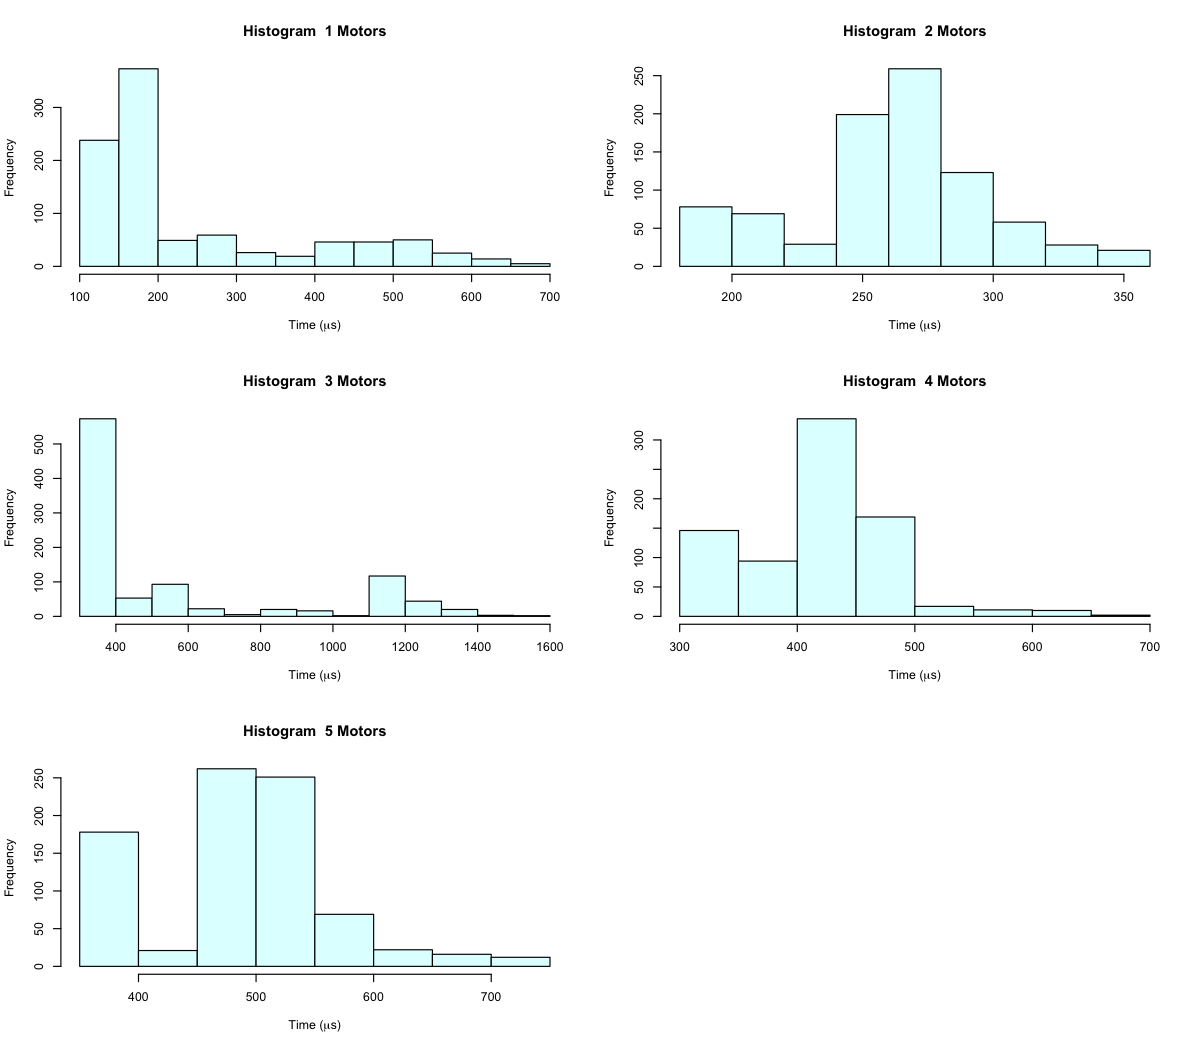
\includegraphics[width=1.0\textwidth]{evaluation/graphics/Droid/Galaxy/HistMotorsDroidGalaxy.png} 
    \caption[Histogramas de motores Droid-Galaxy]{Histogramas de motores  Droid-Galaxy\\Fuente: elaboración propia (2018)} 
    \label{fig:droid-galaxy-hist-motors}
  \end{center}
\end{figure}

\begin{figure}[H]
  \begin{center} 
   	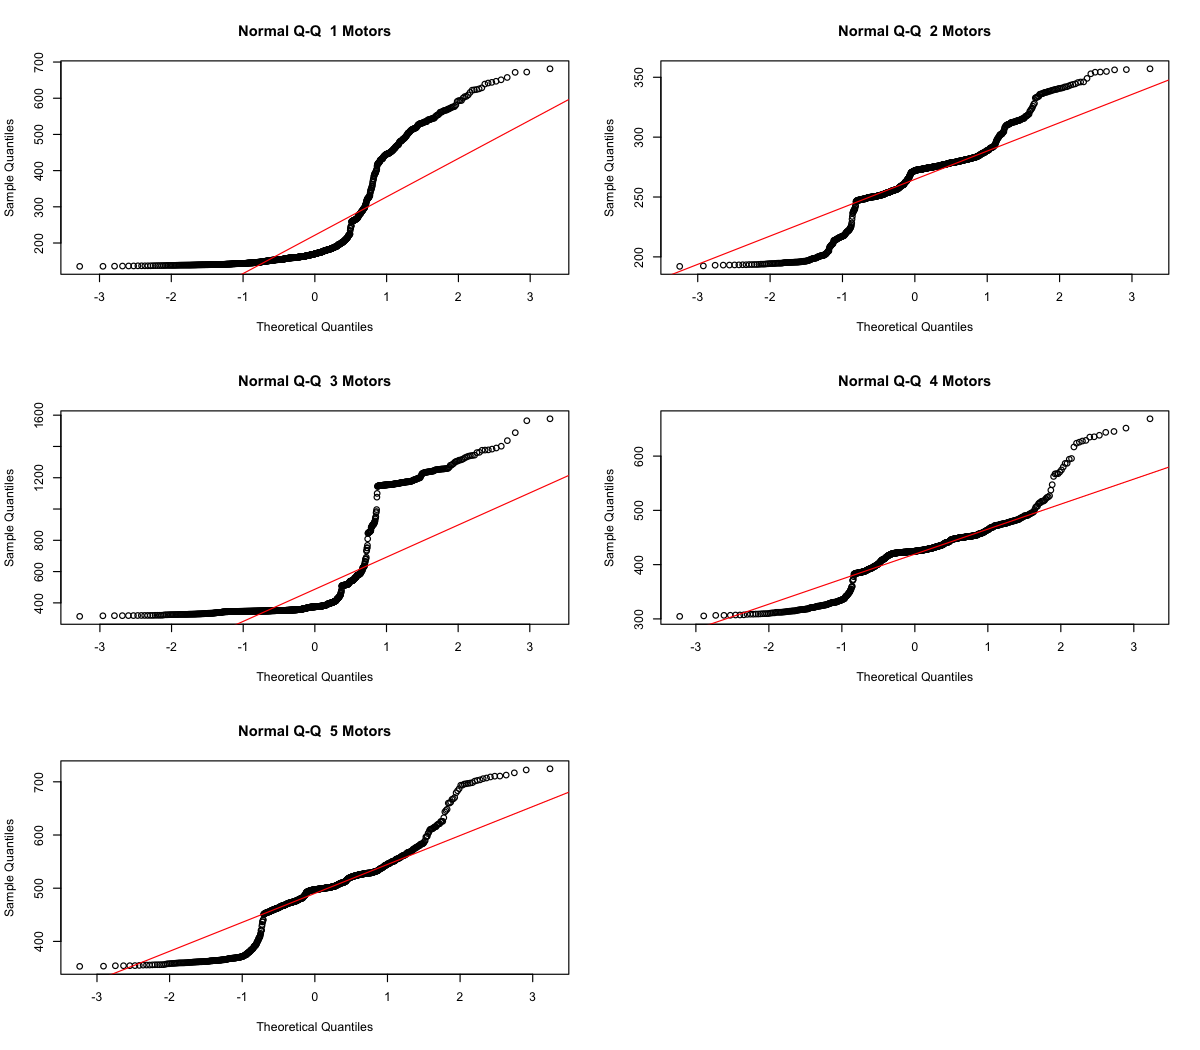
\includegraphics[width=1.0\textwidth]{evaluation/graphics/Droid/Galaxy/NormalQQMotorsDroidGalaxy.png} 
    \caption[Gráfico QQ de motores Droid-Galaxy]{Gráficos QQ de motores Droid-Galaxy\\Fuente: elaboración propia (2018)} 
    \label{fig:droid-galaxy-QQ-motors}
  \end{center}
\end{figure}

\begin{figure}[H]
  \begin{center} 
   	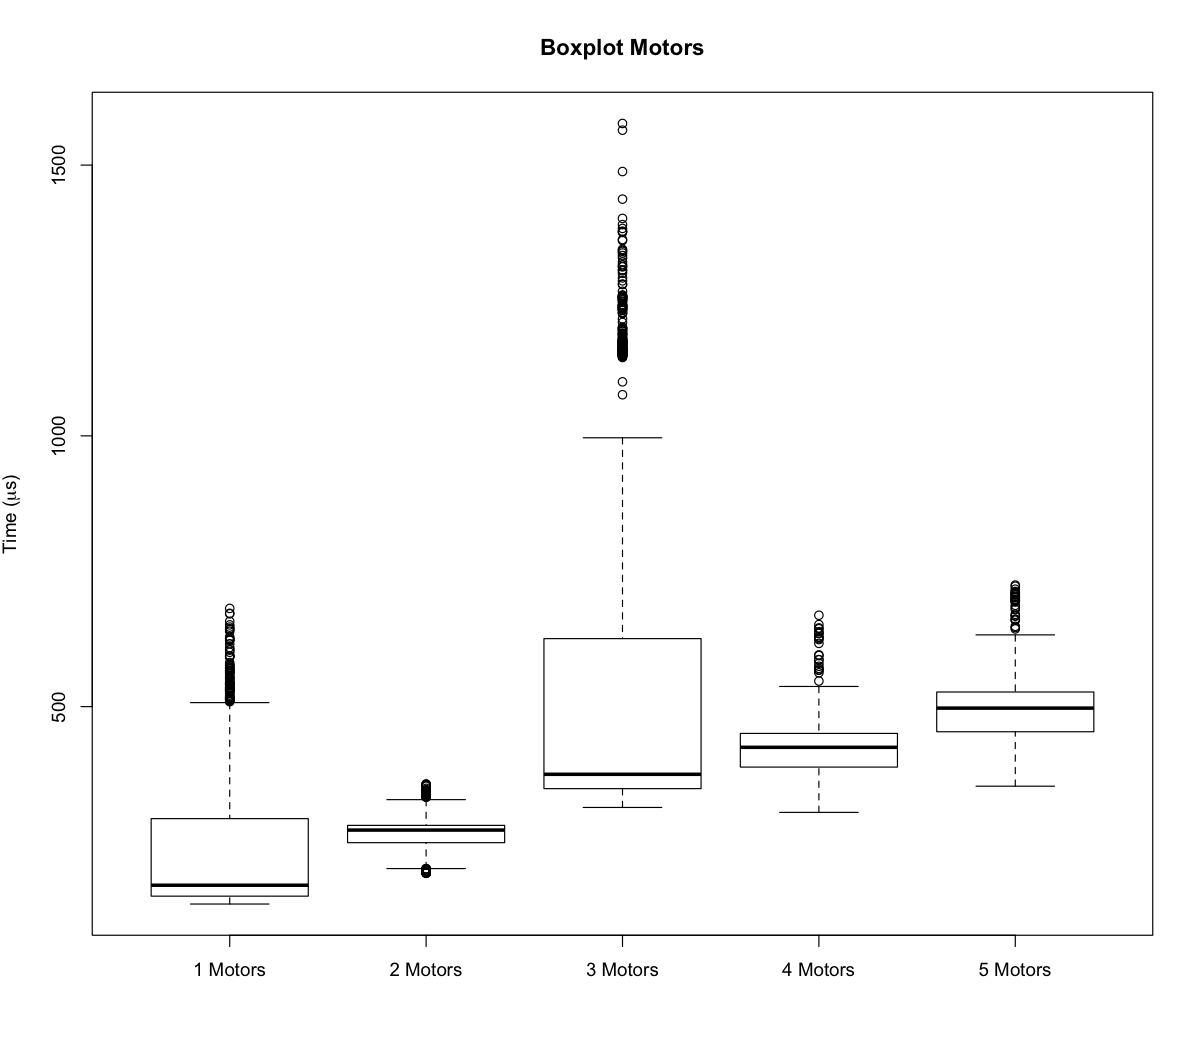
\includegraphics[width=0.8\textwidth]{evaluation/graphics/Droid/Galaxy/BoxplotMotorsDroidGalaxy.png} 
    \caption[Gráficos de cajas de motores Droid-Galaxy]{Gráficos de cajas de motores Droid-Galaxy\\Fuente: elaboración propia (2018)} 
    \label{fig:droid-galaxy-boxplot-motors}
  \end{center}
\end{figure}



\subsubsection{Flexores}

\begin{figure}
 \begin{center} 
   	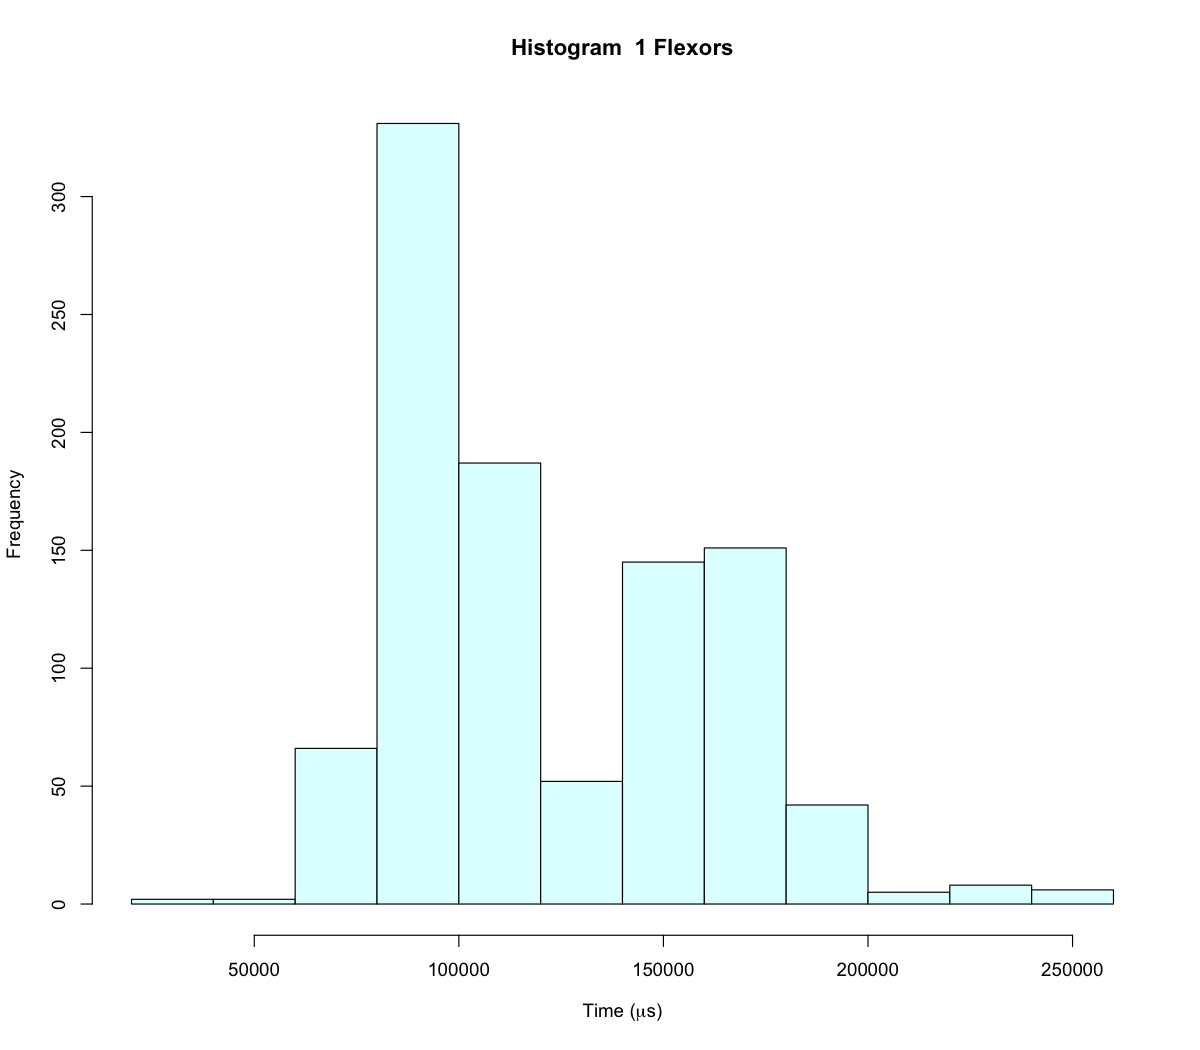
\includegraphics[width=0.5\textwidth]{evaluation/graphics/Droid/Galaxy/HistFlexorsDroidGalaxy.png} 
    \caption[Histogramas de flexores Droid-Galaxy]{Histogramas de flexores  Droid-Galaxy\\Fuente: elaboración propia (2018)} 
    \label{fig:droid-galaxy-hist-flexors}
  \end{center}
\end{figure}

\begin{figure}[H]
  \begin{center} 
   	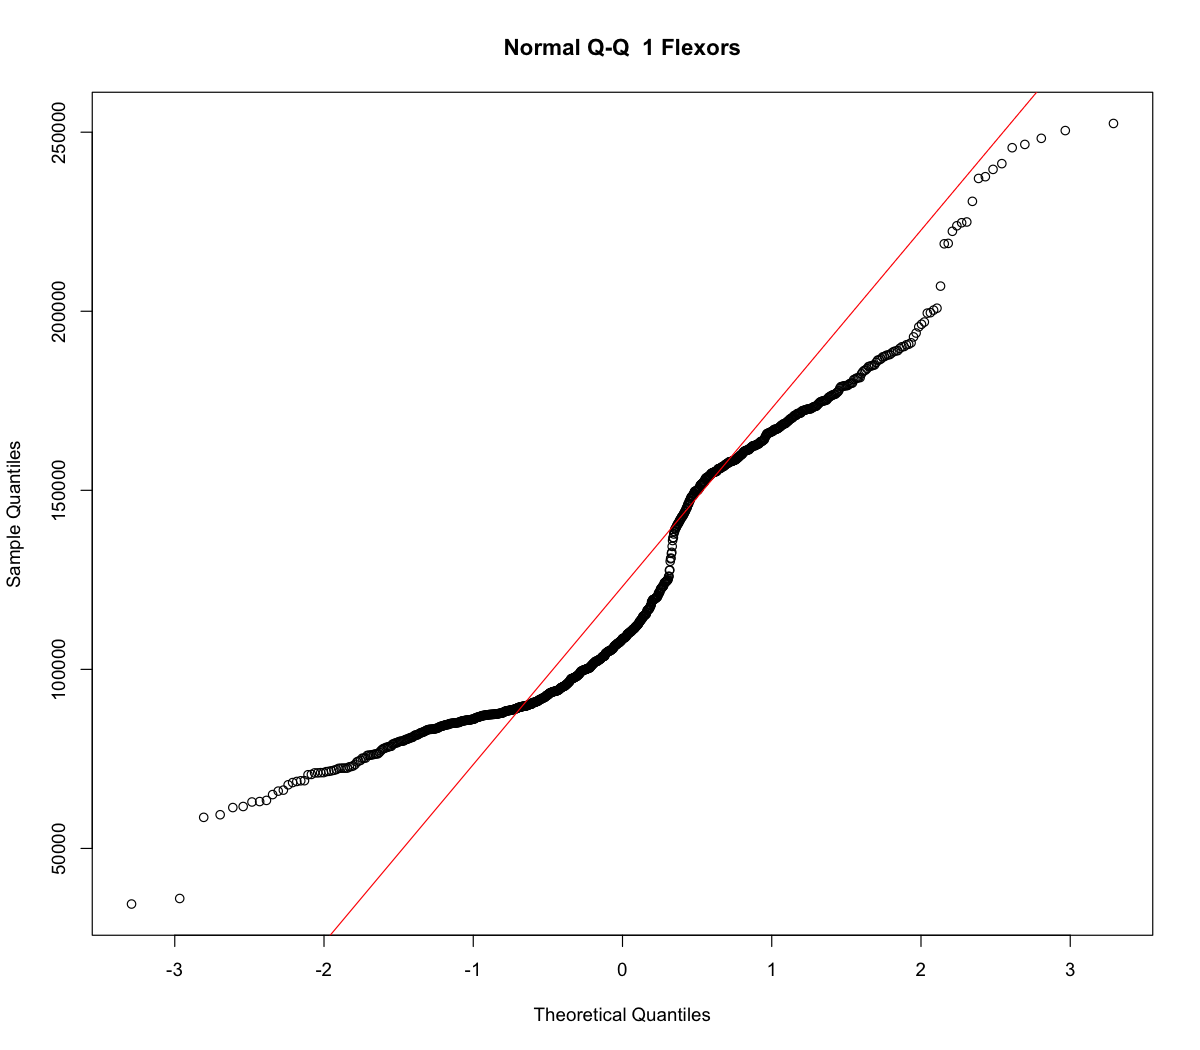
\includegraphics[width=0.5\textwidth]{evaluation/graphics/Droid/Galaxy/NormalQQFlexorsDroidGalaxy.png} 
    \caption[Gráfico QQ de flexores Droid-Galaxy]{Gráficos QQ de flexores Droid-Galaxy\\Fuente: elaboración propia (2018)} 
    \label{fig:droid-galaxy-QQ-flexors}
  \end{center}
\end{figure}

\begin{figure}[H]
  \begin{center} 
   	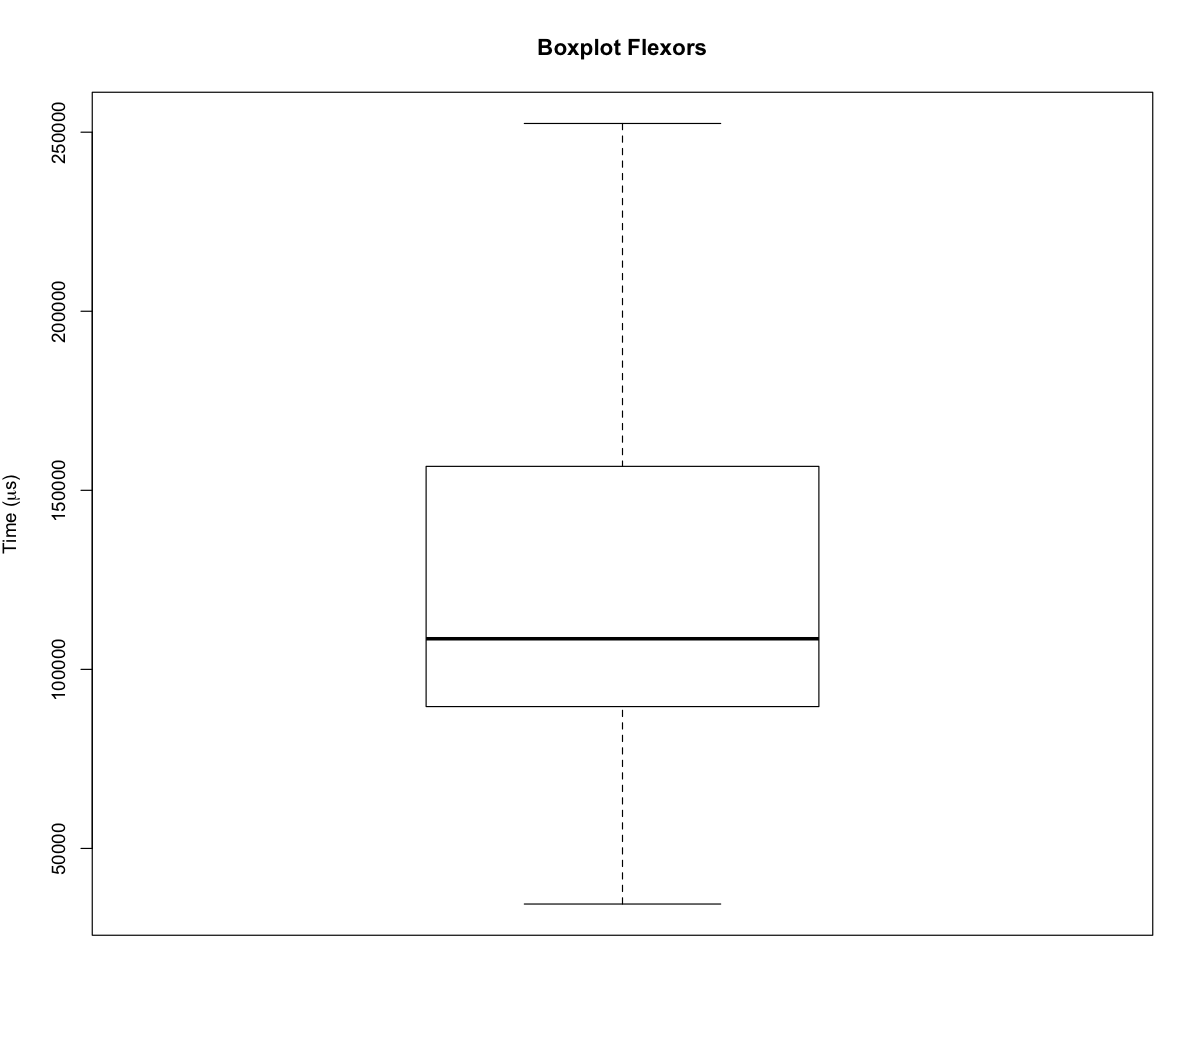
\includegraphics[width=0.5\textwidth]{evaluation/graphics/Droid/Galaxy/BoxplotFlexorsDroidGalaxy.png} 
    \caption[Gráficos de cajas de flexores Droid-Galaxy]{Gráficos de cajas de flexores Droid-Galaxy\\Fuente: elaboración propia (2018)} 
    \label{fig:droid-galaxy-boxplot-flexors}
  \end{center}
\end{figure}


\subsection{Prototipo 4: Xamarin - Galaxy}

\subsubsection{Motores}

\begin{figure}
 \begin{center} 
   	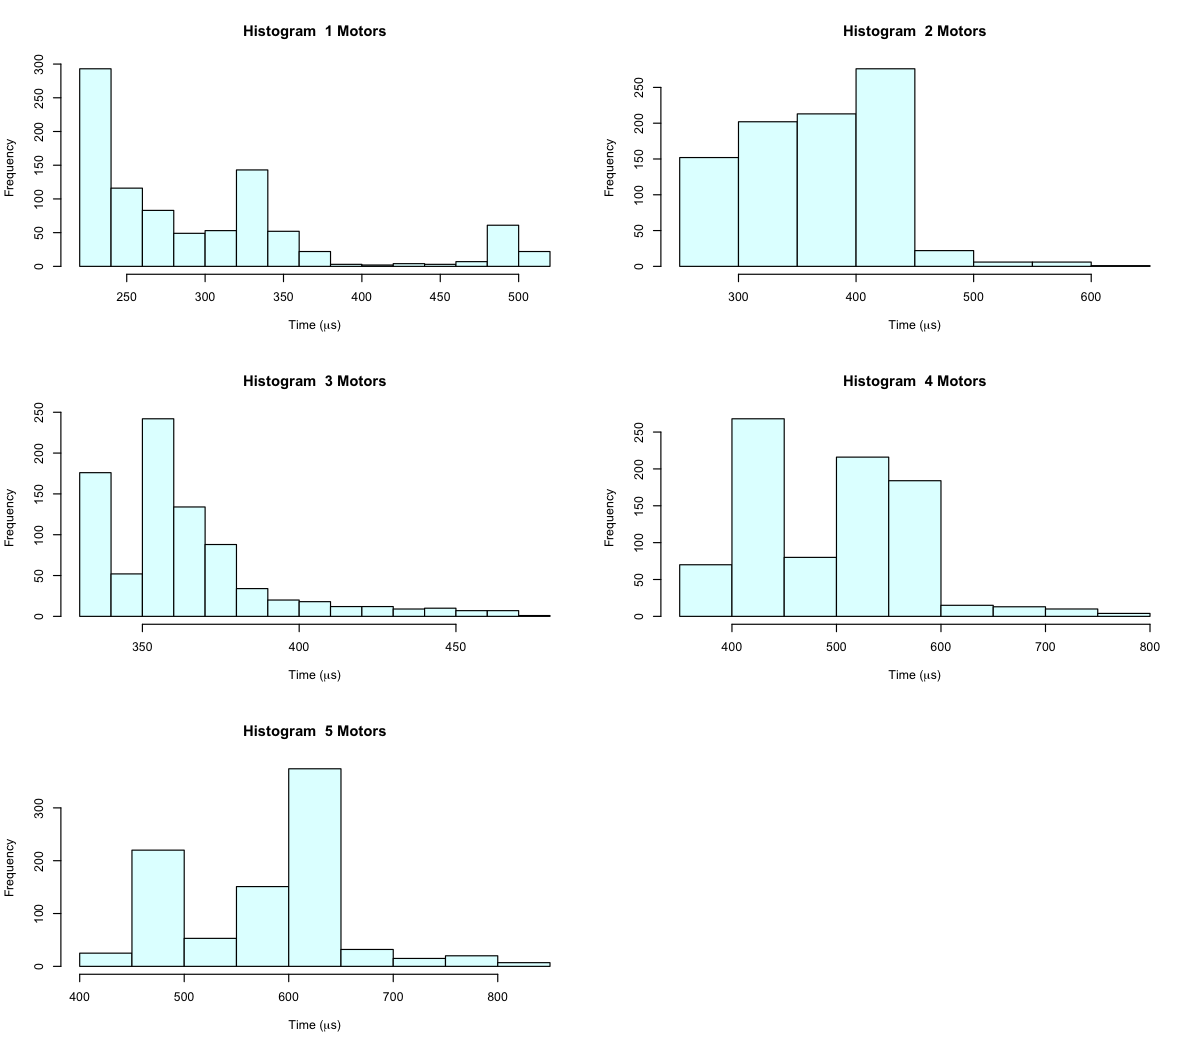
\includegraphics[width=1.0\textwidth]{evaluation/graphics/Xamarin/Galaxy/HistMotorsXamarinGalaxy.png} 
    \caption[Histogramas de motores Xamarin-Galaxy]{Histogramas de motores  Xamarin-Galaxy\\Fuente: elaboración propia (2018)} 
    \label{fig:xamarin-galaxy-hist-motors}
  \end{center}
\end{figure}

\begin{figure}[H]
  \begin{center} 
   	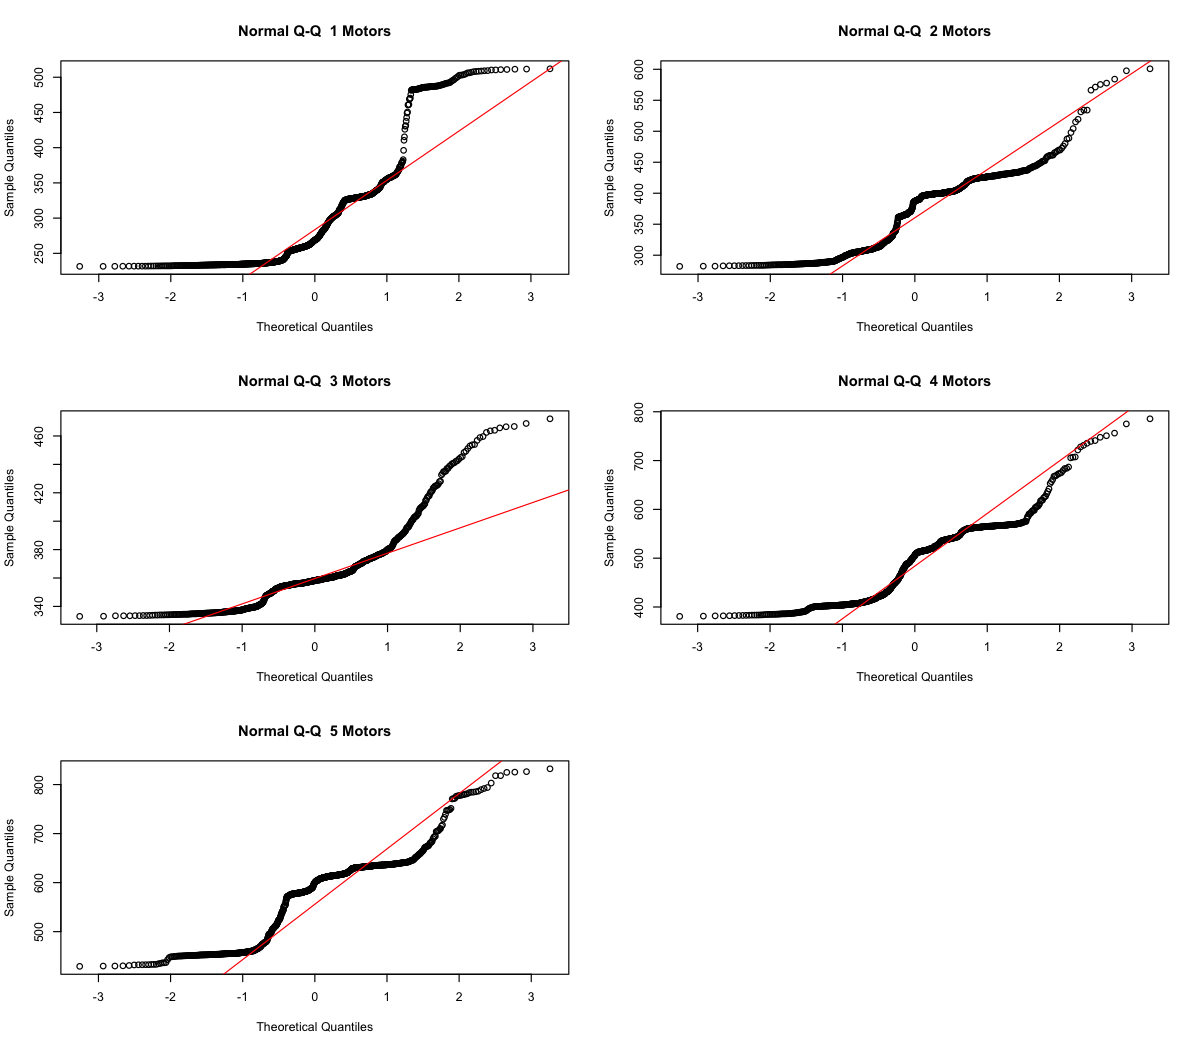
\includegraphics[width=1.0\textwidth]{evaluation/graphics/Xamarin/Galaxy/NormalQQMotorsXamarinGalaxy.png} 
    \caption[Gráfico QQ de motores Xamarin-Galaxy]{Gráficos QQ de motores Xamarin-Galaxy\\Fuente: elaboración propia (2018)} 
    \label{fig:xamarin-galaxy-QQ-motors}
  \end{center}
\end{figure}

\begin{figure}[H]
  \begin{center} 
   	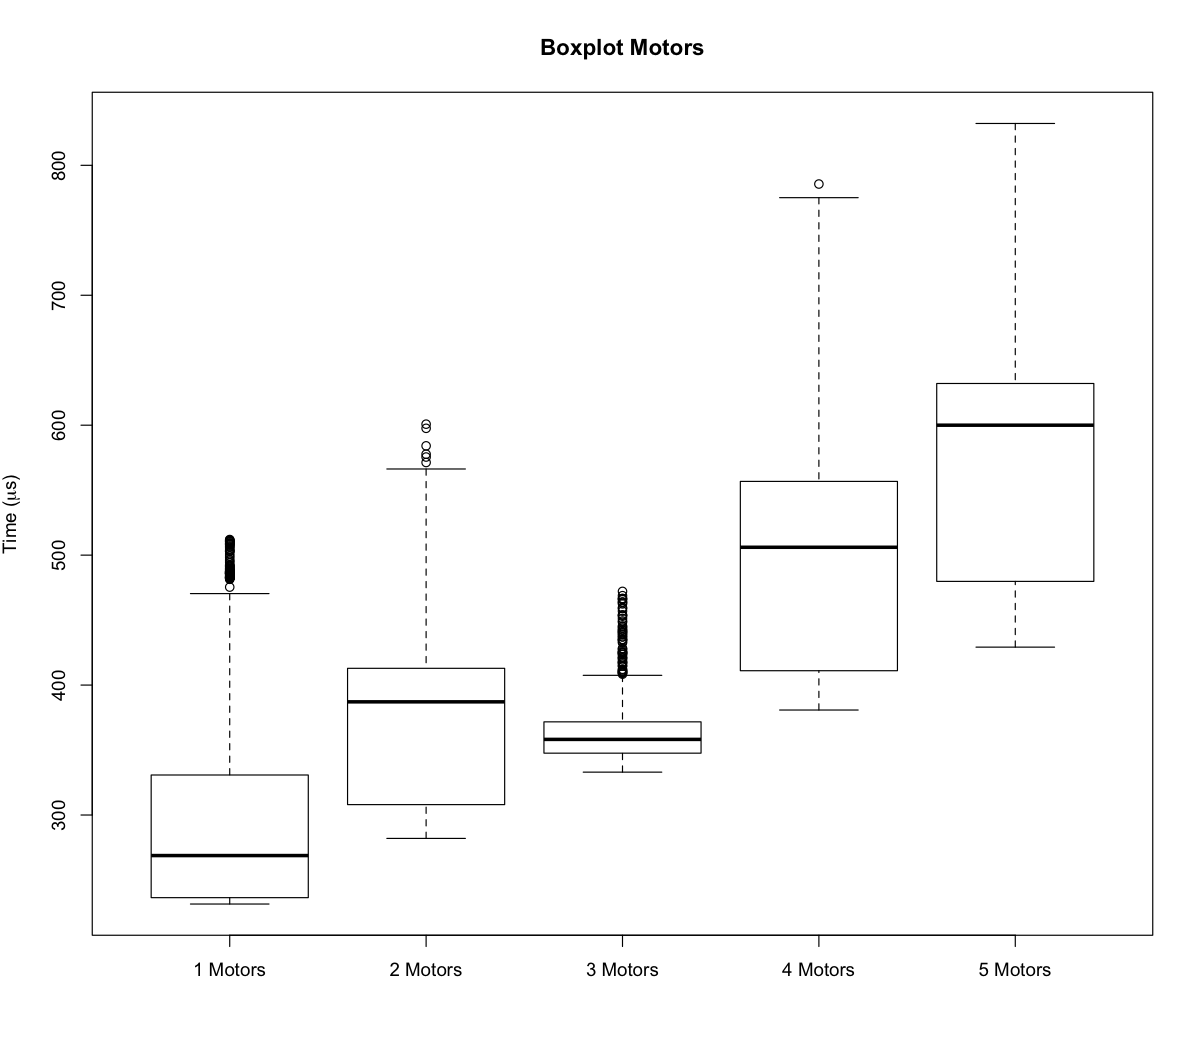
\includegraphics[width=0.8\textwidth]{evaluation/graphics/Xamarin/Galaxy/BoxplotMotorsXamarinGalaxy.png} 
    \caption[Gráficos de cajas de motores Xamarin-Galaxy]{Gráficos de cajas de motores Xamarin-Galaxy\\Fuente: elaboración propia (2018)} 
    \label{fig:xamarin-galaxy-boxplot-motors}
  \end{center}
\end{figure}

\subsubsection{Flexores}

\begin{figure}
 \begin{center} 
   	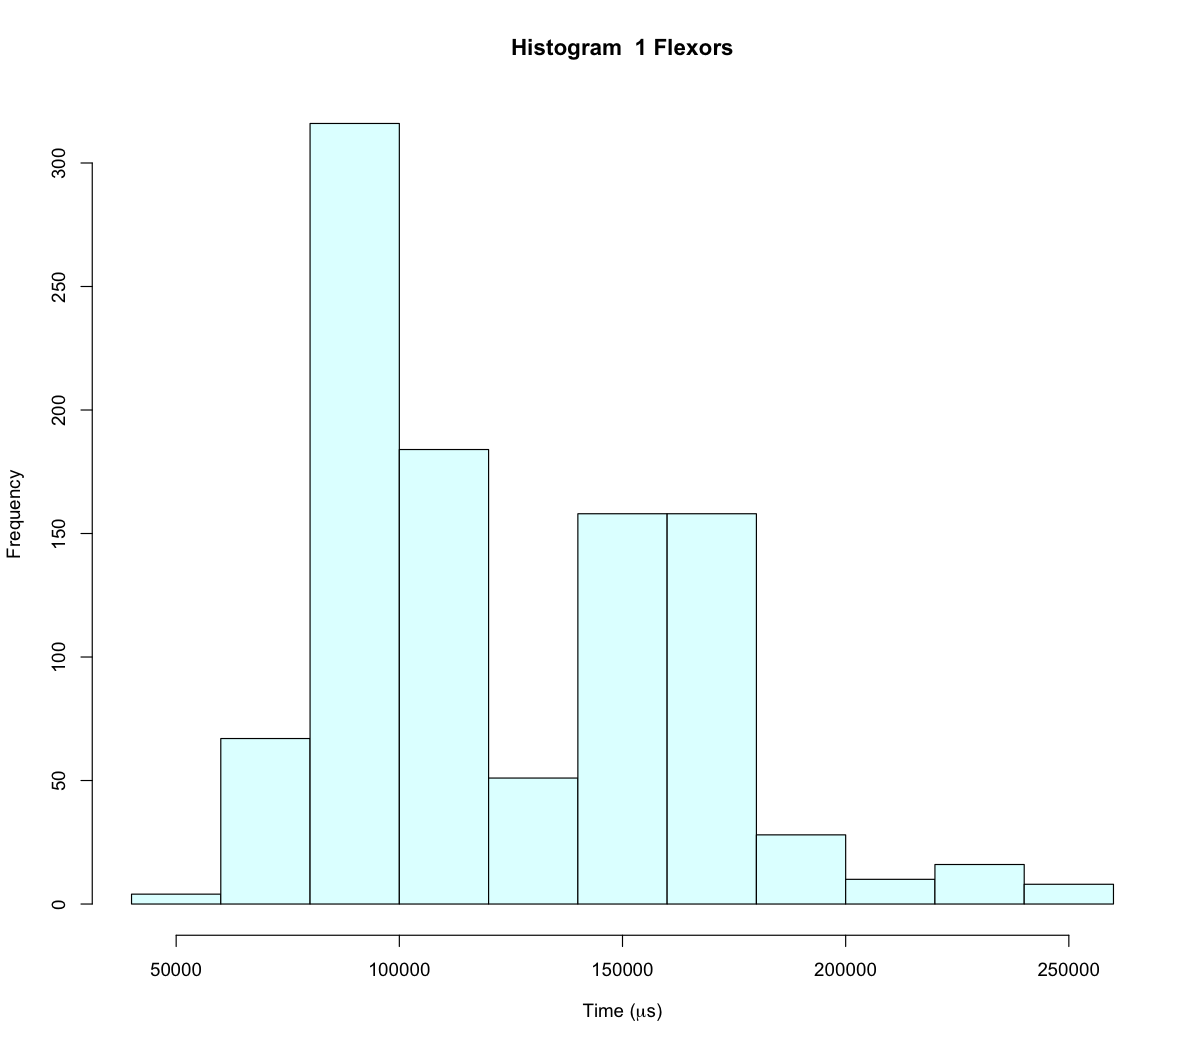
\includegraphics[width=0.5\textwidth]{evaluation/graphics/Xamarin/Galaxy/HistFlexorsXamarinGalaxy.png} 
    \caption[Histogramas de flexores Xamarin-Galaxy]{Histogramas de flexores Xamarin-Galaxy\\Fuente: elaboración propia (2018)} 
    \label{fig:xamarin-galaxy-hist-flexors}
  \end{center}
\end{figure}

\begin{figure}[H]
  \begin{center} 
   	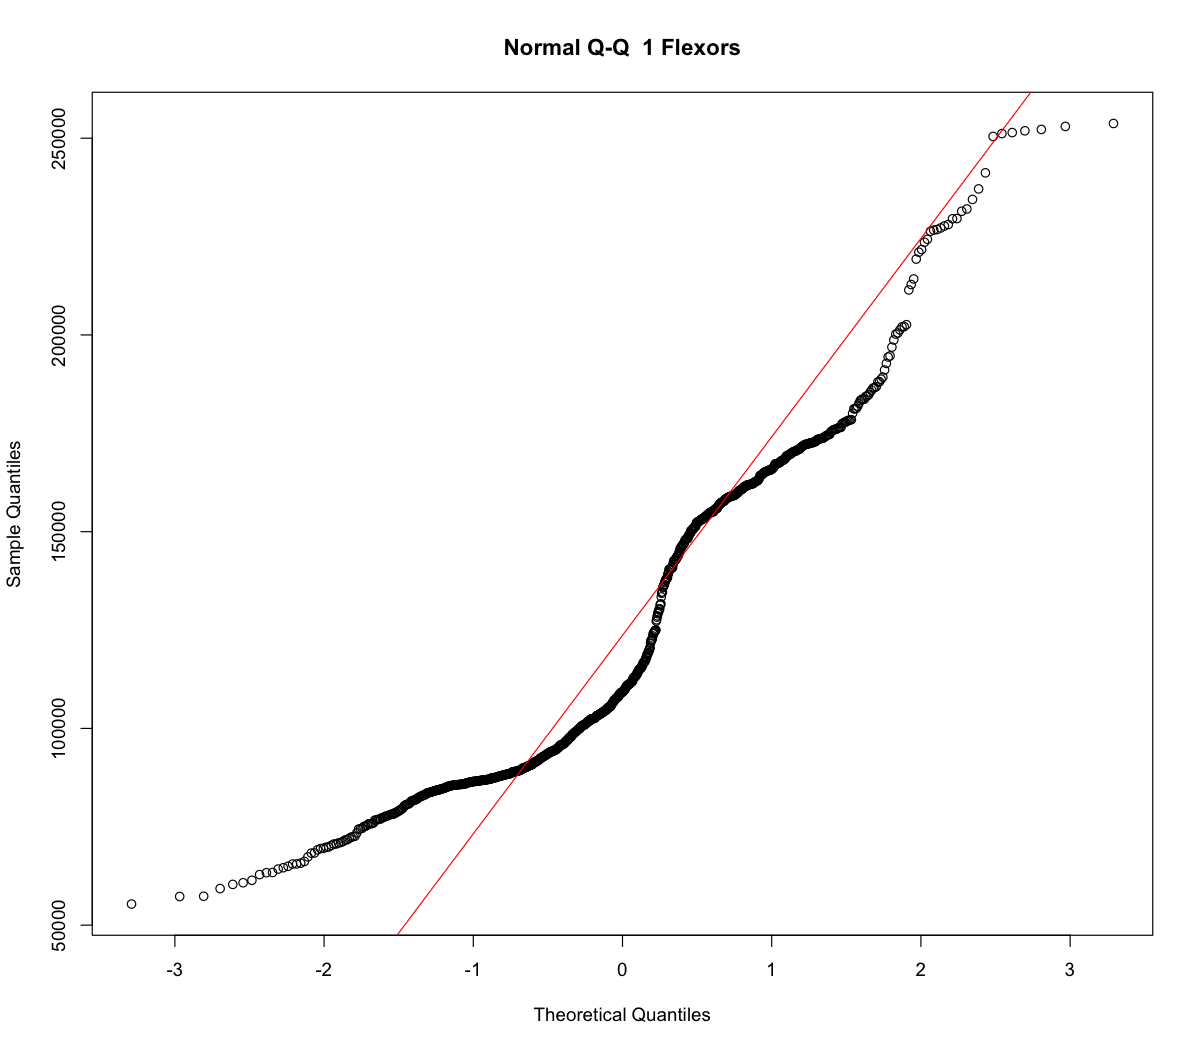
\includegraphics[width=0.5\textwidth]{evaluation/graphics/Xamarin/Galaxy/NormalQQFlexorsXamarinGalaxy.png} 
    \caption[Gráfico QQ de flexores Xamarin-Galaxy]{Gráficos QQ de flexores Xamarin-Galaxy\\Fuente: elaboración propia (2018)} 
    \label{fig:xamarin-galaxy-QQ-flexors}
  \end{center}
\end{figure}

\begin{figure}[H]
  \begin{center} 
   	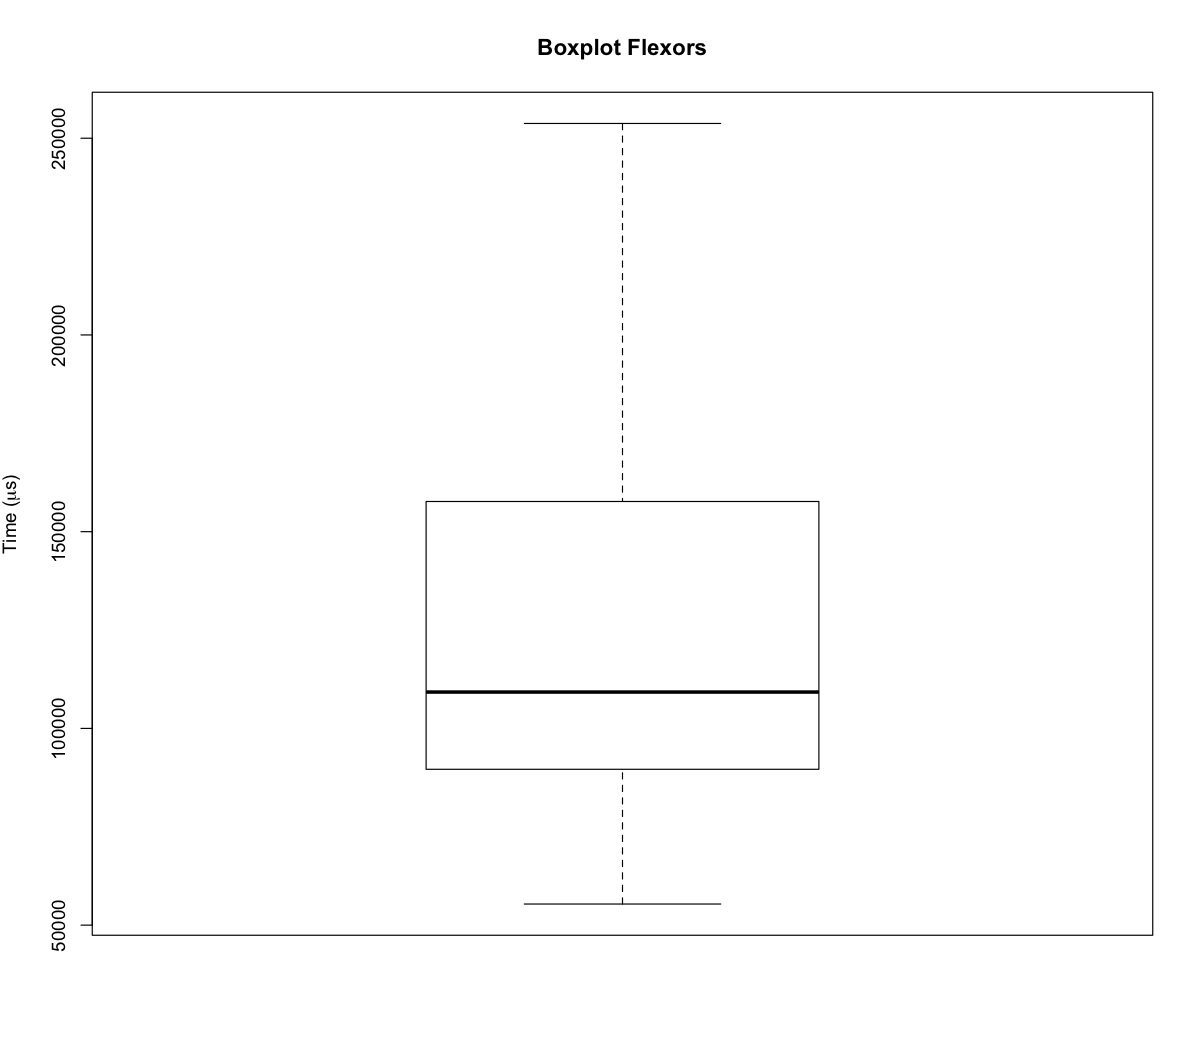
\includegraphics[width=0.5\textwidth]{evaluation/graphics/Xamarin/Galaxy/BoxplotFlexorsXamarinGalaxy.png} 
    \caption[Gráficos de cajas de flexores Xamarin-Galaxy]{Gráficos de cajas de flexores Xamarin-Galaxy\\Fuente: elaboración propia (2018)} 
    \label{fig:xamarin-galaxy-boxplot-flexors}
  \end{center}
\end{figure}


\subsection{Prototipo 3 : Droid - Nexus}

\subsubsection{Motores}

\subsubsection{Flexores}


\subsection{Prototipo 4: Xamarin - Nexus}

\subsubsection{Motores}

\subsubsection{Flexores}